\documentclass[12pt,a4paper]{article}

\usepackage[utf8]{inputenc}
\usepackage[T1]{fontenc}
\usepackage{amsmath,amssymb,amsthm}
\usepackage{booktabs}
\usepackage{array}
\usepackage{graphicx}
\usepackage[margin=1in]{geometry}
\usepackage{hyperref}
\usepackage{setspace}
\onehalfspacing

\newtheorem{assumption}{Assumption}
\newtheorem{proposition}{Proposition}
\newtheorem{remark}{Remark}
\newcommand{\E}{\mathbb{E}}
\newcommand{\Var}{\mathbb{V}\mathrm{ar}}
\newcommand{\Cov}{\mathbb{C}\mathrm{ov}}
\newcommand{\Corr}{\mathbb{C}\mathrm{orr}}
\newcommand{\SR}{\mathrm{SR}}
\newcommand{\UVIF}{\mathrm{UVIF}}
\DeclareMathOperator{\sign}{sign}

\title{Technical Appendix: Sharpe-ratio variance inflation in entity-time financial panels}
\author{Dhananjay S. Chauhan}
\date{June 1, 2026}

\begin{document}
\maketitle

\section{Purpose}

This appendix contains proof details and secondary empirical artifacts
that are omitted from the journal-facing main manuscript for length.
The main manuscript is the claim boundary; this appendix is the audit
trail for derivations, positive controls, robustness tables, and
generated public-data artifacts.

\section{Mean-Return Design-Effect Proof}

For a selected row model \(y_{t,i}=\mu+\lambda_t+\epsilon_{t,i}\) with
constant selected count \(\bar n\), same-date intraclass correlation
\(\rho\), and independent dates, the row-pooled mean equals the average
of date means:
\[
  \hat\mu =
  \frac{1}{T\bar n}\sum_{t=1}^{T}\sum_{i=1}^{\bar n} y_{t,i}
  =
  \frac{1}{T}\sum_{t=1}^{T}\bar y_t .
\]
The row-naive variance report is \(\sigma^2/(T\bar n)\).  The true
one-date variance is
\[
  \Var(\bar y_t)
  =
  \frac{1}{\bar n^2}
  \{\bar n\sigma^2+\bar n(\bar n-1)\rho\sigma^2\}
  =
  \frac{\sigma^2}{\bar n}\{1+(\bar n-1)\rho\}.
\]
Thus
\[
  \frac{se_{date,true}}{se_{row,naive}}
  =
  \sqrt{1+(\bar n-1)\rho}.
\]
This is the Moulton-like design effect used as the mean-return special
case in the main text.

\section{Sharpe UVIF Derivation}

Let \(R_t\) be the date-level portfolio excess return and
\(G_t=(R_t,R_t^2)'\).  The annualized Sharpe ratio is the smooth
functional
\[
  f(\mu,m_2)=\sqrt{252}\frac{\mu}{(m_2-\mu^2)^{1/2}},
  \qquad
  d_R=\nabla f(\mu_R,m_{2,R}).
\]
On sets where \(v_R=m_{2,R}-\mu_R^2>0\), the first-order expansion is
\[
  \widehat{\SR}_R-\SR_R
  =
  d_R'(\hat\theta_R-\theta_R)+o_p(T_R^{-1/2}),
  \qquad \theta_R=\E[G_t].
\]
With long-run covariance
\(\Omega_R=\Gamma_0^R+\sum_{k\ge1}(\Gamma_k^R+\Gamma_k^{R\prime})\),
\[
  \Var_{LR}(\widehat{\SR}_R)
  =
  T_R^{-1}d_R'\Omega_Rd_R+o(T_R^{-1}).
\]
The row-pooled IID calculation applies the same delta method to
\(\bar nT_R\) row observations \(H_{t,i}=(Y_{t,i},Y_{t,i}^2)'\):
\[
  \Var_{IID,row}(\widehat{\SR}_{row})
  =
  (\bar nT_R)^{-1}d_Y'\Psi_Yd_Y+o((\bar nT_R)^{-1}).
\]
Taking the ratio gives the Sharpe UVIF:
\[
  \UVIF_{\SR}
  =
  \frac{\bar n\,d_R'\Omega_Rd_R}{d_Y'\Psi_Yd_Y}
  =
  \frac{\bar n\,d_R'\Gamma_0^Rd_R}{d_Y'\Psi_Yd_Y}
  \times
  \frac{d_R'\Omega_Rd_R}{d_R'\Gamma_0^Rd_R}.
\]
The first term is the cross-sectional component and the second term is
the serial long-run factor.  Componentwise,
\[
  d_R'\Omega_Rd_R
  =
  \frac{252}{v_R^3}
  \left[
    m_{2,R}^2\Omega_{11}
    -\frac{\mu_Rm_{2,R}}{2}(\Omega_{12}+\Omega_{21})
    +\frac{\mu_R^2}{4}\Omega_{22}
  \right].
\]
The \(\Omega_{22}\) term contains long-run covariances of squared
returns and therefore brings fourth moments into Sharpe-ratio variance.

\section{Capacity stress extension}

The public sorted-portfolio examples in the main manuscript do not
contain average daily volume or order-size information, so they do not
support a capacity claim.  For traded-security panels where those inputs
are available, a square-root impact diagnostic can be added as an
extension to the statistical claim boundary.

\begin{proposition}[Asymptotic capacity frontier under square-root impact]
\label{prop:capacity-frontier}
Suppose a traded panel has row-pooled gross mean \(\bar r_{\mathrm{gross}}\),
row-pooled return standard deviation \(\sigma_{\mathrm{row}}\), average turnover
\(\widehat{TO}>0\), \(T\) trading dates, square-root impact cost
\(\lambda \widehat{TO}\sqrt{A/V}\), and a dependence standard-error
inflation factor \(\mathcal M\ge 1\) relative to row-pooled inference.
For a one-sided level-\(\alpha\) viability margin, any statistically
certified capacity \(A^*\) must satisfy
\begin{equation}
  A^*
  \le
  V\left(
    \frac{\bar r_{\mathrm{gross}}
      -z_{\alpha}\mathcal M\sigma_{\mathrm{row}}/\sqrt{T}}
         {\lambda \widehat{TO}}
  \right)^2
  \label{eq:capacity-frontier}
\end{equation}
when the numerator is positive; otherwise no positive capacity is
certified by the margin.
\end{proposition}

For a square-root impact diagnostic, the dependence-adjusted one-sided
lower confidence margin for gross mean return is
\[
  \bar r_{\mathrm{gross}}
  - z_{\alpha}\mathcal M\sigma_{\mathrm{row}}/\sqrt{T},
\]
where \(\sigma_{\mathrm{row}}\) is the standard deviation of row-pooled
returns before date aggregation or UVIF adjustment.  Square-root impact
subtracts \(\lambda\widehat{TO}\sqrt{A/V}\).  Requiring the net lower
margin to be nonnegative gives
\[
  \lambda\widehat{TO}\sqrt{A/V}
  \le
  \bar r_{\mathrm{gross}}
  - z_{\alpha}\mathcal M\sigma_{\mathrm{row}}/\sqrt{T}.
\]
Rearranging yields the capacity frontier in Proposition
\ref{prop:capacity-frontier}.  If
the volatility input is already the date-level portfolio volatility, the
date boundary has already embedded the cross-sectional UVIF component,
so the cross-sectional part of \(\mathcal M\) must not be multiplied in
again.

\section{Higher-Moment UVIF and ERIR Details}

For \(\theta^{(4)}=(\mu,m_2,m_3,m_4)'\), define skewness and kurtosis
from the central moments implied by \(\theta^{(4)}\).  Any adjusted
Sharpe functional \(h(\theta^{(4)})\) has a delta-method variance
\(\nabla h'\Omega^{(4)}\nabla h\), where \(\Omega^{(4)}\) is the
long-run covariance matrix of \((R_t,R_t^2,R_t^3,R_t^4)'\).  The
higher-moment UVIF is the corresponding ratio of date-level long-run
variance to row-pooled IID variance.  It is a diagnostic extension, not
an additional empirical rejection gate.

The Effective Row Information Retention (ERIR) diagnostic is a
design-effect retention calculation, not a hypothesis test or a formal
information claim.  Under the same equicorrelated approximation
used for the mean-return design effect,
\[
  DE_{\mu,xs}=1+(\bar n-1)\rho,
  \qquad
  \mathrm{ERIR}=\{1+(\bar n-1)\rho\}^{-1}.
\]
Thus an ERIR of \(0.111\) means that roughly \(1-0.111=0.889\), or 89
percent, of nominal row-level information is redundant under this
diagnostic approximation.  Confirmatory inference remains based on
date-level HAC-delta and dependent-bootstrap procedures.

\section{Synthetic Positive Control}

\begin{table}[t]
\centering
\small
\caption{Synthetic positive-control audit.}
\label{tab:synthetic-positive-control}
\begin{tabular}{lrrrrrr}
\toprule
Panel & $\bar\rho$ & Adj. & SR & HAC $p^+$ & RW $p$ & Perm. $p^+$ \\
\midrule
Synthetic control & 0.202 & 4.58 & 1.744 & 7.67e-13 & 5.00e-04 & 9.99e-04 \\
\bottomrule
\end{tabular}
\end{table}


\section{Full Empirical Artifacts}

The inferential tables in this appendix report only public sources that
loaded and produced reproducible artifacts.  Failed source-access
attempts remain in the generated provenance files and campaign metadata,
but are not treated as empirical evidence.

% Generated by render_manuscript_artifacts.py from campaign root code/output_overhaul_20260601
\begin{table}[t]
\centering
\small
\caption{Registry-defined public candidate evaluation campaign.}
\label{tab:candidate-campaign}
\resizebox{\textwidth}{!}{%
\begin{tabular}{lllllllll}
\toprule
Candidate & status & SR & HAC p+ & Boot p+ & RW p & Perm p & Net SR & Pass 5\% \\
\midrule
french\_momentum\_deciles\_daily\_rank & Available & 0.447 & 7.54e-05 & 2.00e-04 & 2.00e-04 & 1.000 & 0.447 & no \\
french\_momentum\_deciles\_daily\_wml & Available & 0.497 & 5.53e-06 & 2.00e-04 & 2.00e-04 & 1.00e-04 & 0.497 & yes \\
french\_size\_bm\_daily\_dynamic\_momentum & Available & 0.036 & 0.445 & 0.458 & 0.516 & 0.947 & -0.072 & no \\
stooq\_fixed\_etf\_daily\_dynamic\_momentum & Data unavailable &  &  &  &  &  &  & no \\
aqr\_bab\_equity\_factors\_daily & Available & 0.741 & 3.08e-13 & 2.00e-04 & 2.00e-04 &  & 0.741 & no \\
aqr\_qmj\_factors\_daily & Available & 0.536 & 2.26e-05 & 2.00e-04 & 2.00e-04 &  & 0.536 & no \\
aqr\_hml\_devil\_factors\_daily & Available & 0.336 & 0.004 & 0.002 & 0.002 &  & 0.336 & no \\
aqr\_value\_momentum\_everywhere\_monthly & Available & 2.623 & 1.62e-04 & 2.00e-04 & 2.00e-04 &  & 2.623 & no \\
\bottomrule
\end{tabular}%
}
\end{table}

\begin{table}[t]
\centering
\small
\caption{Canonical French momentum benchmark validation.}
\label{tab:momentum-benchmark}
\resizebox{\textwidth}{!}{%
\begin{tabular}{llllllll}
\toprule
Candidate & thr & n & start & end & panel SR & direct WML SR & scale \\
\midrule
french\_momentum\_deciles\_daily\_wml & 0.900 & 26131 & 1926-11-04 & 2026-04-30 & 0.497 & 0.497 & 0.500 \\
\bottomrule
\end{tabular}%
}
\end{table}

\begin{table}[t]
\centering
\small
\caption{Sampling-boundary design-effect diagnostics.}
\label{tab:row-boundary}
\resizebox{\textwidth}{!}{%
\begin{tabular}{lllllllllllll}
\toprule
Candidate & status & thr & rows & dates & avg names & rho & SE infl. & row t & HAC z & row p+ & HAC p+ & RW p \\
\midrule
aqr\_bab\_equity\_factors\_daily & not\_applicable\_single\_series & 0.000 & 25281 & 25281 & 1.000 &  &  &  &  &  &  & 2.00e-04 \\
aqr\_hml\_devil\_factors\_daily & not\_applicable\_single\_series & 0.000 & 26590 & 26590 & 1.000 &  &  &  &  &  &  & 0.002 \\
aqr\_qmj\_factors\_daily & not\_applicable\_single\_series & 0.000 & 17681 & 17681 & 1.000 &  &  &  &  &  &  & 2.00e-04 \\
aqr\_value\_momentum\_everywhere\_monthly & not\_applicable\_single\_series & 0.000 & 651 & 651 & 1.000 &  &  &  &  &  &  & 2.00e-04 \\
french\_momentum\_deciles\_daily\_rank & Available & 0.700 & 104524 & 26131 & 4.000 & -0.138 & 0.766 & 3.584 & 3.790 & 1.70e-04 & 7.54e-05 & 2.00e-04 \\
french\_momentum\_deciles\_daily\_wml & Available & 0.900 & 52262 & 26131 & 2.000 & -0.583 & 0.646 & 3.299 & 4.395 & 4.85e-04 & 5.53e-06 & 2.00e-04 \\
french\_size\_bm\_daily\_dynamic\_momentum & Available & 0.500 & 45201 & 3477 & 13.000 & 0.667 & 3.000 & 0.664 & 0.222 & 0.253 & 0.412 & 0.516 \\
\bottomrule
\end{tabular}%
}
\end{table}

\begin{table}[t]
\centering
\small
\caption{Dependence audit summary for panel candidates.}
\label{tab:phantom-audit}
\resizebox{\textwidth}{!}{%
\begin{tabular}{lllllll}
\toprule
Candidate & Row p+ & UVIF & EIR & Audit p+ & Net SR & Status \\
\midrule
french\_momentum\_deciles\_daily\_rank & 1.70e-04 & 1.000 & 1.000 & 1.000 & 0.447 & Fails permutation gate \\
french\_momentum\_deciles\_daily\_wml & 4.85e-04 & 1.000 & 1.000 & 2.00e-04 & 0.497 & Passes composite gate \\
french\_size\_bm\_daily\_dynamic\_momentum & 0.253 & 9.002 & 0.111 & 0.947 & -0.072 & Fails cost gate \\
\bottomrule
\end{tabular}%
}
\par\footnotesize\emph{Note:} EIR is a diagnostic approximation and is not used as a rejection rule.
\end{table}

\begin{table}[t]
\centering
\small
\caption{Horizon-effect audit for the dynamic Size/BM momentum panel.}
\label{tab:horizon-effect}
\resizebox{\textwidth}{!}{%
\begin{tabular}{llllllllll}
\toprule
L & thr & dates & avg names & gross SR & net SR 5bps & turnover & UVIF SR & serial UVIF & HAC p+ \\
\midrule
1 & 0.500 & 3497 & 12.913 & 0.073 & -0.394 & 0.733 & 11.498 & 0.891 & 0.386 \\
5 & 0.500 & 3493 & 13.000 & -0.312 & -0.528 & 0.339 & 12.880 & 0.990 & 0.878 \\
21 & 0.500 & 3477 & 13.000 & 0.058 & -0.050 & 0.169 & 12.121 & 0.933 & 0.412 \\
\bottomrule
\end{tabular}%
}
\end{table}

\begin{table}[t]
\centering
\small
\caption{Primary-threshold dependence-aware Sharpe inference.}
\label{tab:empirical-inference}
\resizebox{\textwidth}{!}{%
\begin{tabular}{lllllllll}
\toprule
Candidate & thr & Method & SR & SE & CI low & CI high & p+ & n \\
\midrule
aqr\_bab\_equity\_factors\_daily & 0.000 & block & 0.741 & 0.106 & 0.533 & 0.951 & 2.00e-04 & 25281 \\
aqr\_bab\_equity\_factors\_daily & 0.000 & HAC & 0.741 & 0.103 & 0.540 & 0.943 & 3.08e-13 & 25281 \\
aqr\_bab\_equity\_factors\_daily & 0.000 & prewhite & 0.741 & 0.104 & 0.538 & 0.945 & 4.38e-13 & 25281 \\
aqr\_hml\_devil\_factors\_daily & 0.000 & block & 0.336 & 0.114 & 0.105 & 0.552 & 0.002 & 26590 \\
aqr\_hml\_devil\_factors\_daily & 0.000 & HAC & 0.336 & 0.126 & 0.089 & 0.583 & 0.004 & 26590 \\
aqr\_hml\_devil\_factors\_daily & 0.000 & prewhite & 0.336 & 0.111 & 0.119 & 0.553 & 0.001 & 26590 \\
aqr\_qmj\_factors\_daily & 0.000 & block & 0.536 & 0.133 & 0.276 & 0.795 & 2.00e-04 & 17681 \\
aqr\_qmj\_factors\_daily & 0.000 & HAC & 0.536 & 0.131 & 0.279 & 0.794 & 2.26e-05 & 17681 \\
aqr\_qmj\_factors\_daily & 0.000 & prewhite & 0.536 & 0.128 & 0.285 & 0.787 & 1.40e-05 & 17681 \\
aqr\_value\_momentum\_everywhere\_monthly & 0.000 & block & 2.623 & 0.716 & 1.230 & 4.041 & 2.00e-04 & 651 \\
aqr\_value\_momentum\_everywhere\_monthly & 0.000 & HAC & 2.625 & 0.730 & 1.194 & 4.056 & 1.62e-04 & 651 \\
aqr\_value\_momentum\_everywhere\_monthly & 0.000 & prewhite & 2.625 & 0.723 & 1.207 & 4.043 & 1.42e-04 & 651 \\
french\_momentum\_deciles\_daily\_rank & 0.700 & block & 0.447 & 0.114 & 0.222 & 0.667 & 2.00e-04 & 26131 \\
french\_momentum\_deciles\_daily\_rank & 0.700 & HAC & 0.447 & 0.118 & 0.216 & 0.679 & 7.54e-05 & 26131 \\
french\_momentum\_deciles\_daily\_rank & 0.700 & prewhite & 0.447 & 0.114 & 0.224 & 0.670 & 4.18e-05 & 26131 \\
french\_momentum\_deciles\_daily\_wml & 0.900 & block & 0.497 & 0.111 & 0.275 & 0.708 & 2.00e-04 & 26131 \\
french\_momentum\_deciles\_daily\_wml & 0.900 & HAC & 0.497 & 0.113 & 0.275 & 0.718 & 5.53e-06 & 26131 \\
french\_momentum\_deciles\_daily\_wml & 0.900 & prewhite & 0.497 & 0.111 & 0.279 & 0.715 & 3.99e-06 & 26131 \\
french\_size\_bm\_daily\_dynamic\_momentum & 0.500 & block & 0.036 & 0.261 & -0.487 & 0.530 & 0.458 & 3477 \\
french\_size\_bm\_daily\_dynamic\_momentum & 0.500 & HAC & 0.036 & 0.260 & -0.473 & 0.544 & 0.445 & 3477 \\
\bottomrule
\end{tabular}%
}
\end{table}

\begin{table}[t]
\centering
\small
\caption{Same-date signal-permutation diagnostics for panel candidates.}
\label{tab:permutation}
\resizebox{\textwidth}{!}{%
\begin{tabular}{lllllll}
\toprule
Candidate & thr & obs SR & null mean & null sd & p+ & perms \\
\midrule
french\_momentum\_deciles\_daily\_rank & 0.000 & 0.395 & 0.410 & 0.039 & 0.646 & 10000 \\
french\_momentum\_deciles\_daily\_rank & 0.300 & 0.419 & 0.434 & 0.024 & 0.733 & 10000 \\
french\_momentum\_deciles\_daily\_rank & 0.500 & 0.419 & 0.434 & 0.024 & 0.733 & 10000 \\
french\_momentum\_deciles\_daily\_rank & 0.700 & 0.447 & 0.447 & 1.11e-16 & 1.000 & 10000 \\
french\_momentum\_deciles\_daily\_rank & 0.900 & 0.497 & 0.404 & 0.042 & 0.015 & 10000 \\
french\_momentum\_deciles\_daily\_wml & 0.900 & 0.497 & -0.001 & 0.098 & 1.00e-04 & 10000 \\
french\_size\_bm\_daily\_dynamic\_momentum & 0.000 & 0.011 & 0.052 & 0.017 & 0.993 & 10000 \\
french\_size\_bm\_daily\_dynamic\_momentum & 0.300 & 0.010 & 0.072 & 0.023 & 0.996 & 10000 \\
french\_size\_bm\_daily\_dynamic\_momentum & 0.500 & 0.036 & 0.083 & 0.029 & 0.947 & 10000 \\
french\_size\_bm\_daily\_dynamic\_momentum & 0.700 & 0.061 & 0.112 & 0.040 & 0.893 & 10000 \\
french\_size\_bm\_daily\_dynamic\_momentum & 0.900 & 0.025 & 0.098 & 0.069 & 0.855 & 10000 \\
\bottomrule
\end{tabular}%
}
\end{table}

\begin{table}[t]
\centering
\small
\caption{HAC bandwidth, prewhitening, and fixed-b robustness diagnostics.}
\label{tab:hac-robustness}
\resizebox{\textwidth}{!}{%
\begin{tabular}{lllll}
\toprule
Candidate & Diagnostic & SR & SE & p+ \\
\midrule
aqr\_bab\_equity\_factors\_daily & HAC K=auto & 0.741 & 0.103 & 3.08e-13 \\
aqr\_bab\_equity\_factors\_daily & HAC K=21 & 0.741 & 0.119 & 2.04e-10 \\
aqr\_bab\_equity\_factors\_daily & HAC K=63 & 0.741 & 0.130 & 6.06e-09 \\
aqr\_bab\_equity\_factors\_daily & prewhite & 0.741 & 0.104 & 4.38e-13 \\
aqr\_bab\_equity\_factors\_daily & fixed-b 0.1 & 0.741 & 0.166 & 0.002 \\
aqr\_hml\_devil\_factors\_daily & HAC K=auto & 0.336 & 0.126 & 0.004 \\
aqr\_hml\_devil\_factors\_daily & HAC K=21 & 0.336 & 0.128 & 0.004 \\
aqr\_hml\_devil\_factors\_daily & HAC K=63 & 0.336 & 0.137 & 0.007 \\
aqr\_hml\_devil\_factors\_daily & prewhite & 0.336 & 0.111 & 0.001 \\
aqr\_hml\_devil\_factors\_daily & fixed-b 0.1 & 0.336 & 0.110 & 0.004 \\
aqr\_qmj\_factors\_daily & HAC K=auto & 0.536 & 0.131 & 2.26e-05 \\
aqr\_qmj\_factors\_daily & HAC K=21 & 0.536 & 0.140 & 6.33e-05 \\
aqr\_qmj\_factors\_daily & HAC K=63 & 0.536 & 0.147 & 1.32e-04 \\
aqr\_qmj\_factors\_daily & prewhite & 0.536 & 0.128 & 1.40e-05 \\
aqr\_qmj\_factors\_daily & fixed-b 0.1 & 0.536 & 0.151 & 0.002 \\
aqr\_value\_momentum\_everywhere\_monthly & HAC K=auto & 2.625 & 0.730 & 1.62e-04 \\
aqr\_value\_momentum\_everywhere\_monthly & HAC K=21 & 2.625 & 0.712 & 1.14e-04 \\
aqr\_value\_momentum\_everywhere\_monthly & HAC K=63 & 2.625 & 0.659 & 3.41e-05 \\
aqr\_value\_momentum\_everywhere\_monthly & prewhite & 2.625 & 0.723 & 1.42e-04 \\
aqr\_value\_momentum\_everywhere\_monthly & fixed-b 0.1 & 2.625 & 0.656 & 0.004 \\
french\_momentum\_deciles\_daily\_rank & HAC K=auto & 0.447 & 0.118 & 7.54e-05 \\
french\_momentum\_deciles\_daily\_rank & HAC K=21 & 0.447 & 0.120 & 9.94e-05 \\
french\_momentum\_deciles\_daily\_rank & HAC K=63 & 0.447 & 0.122 & 1.21e-04 \\
french\_momentum\_deciles\_daily\_rank & prewhite & 0.447 & 0.114 & 4.18e-05 \\
french\_momentum\_deciles\_daily\_rank & fixed-b 0.1 & 0.447 & 0.143 & 0.004 \\
french\_momentum\_deciles\_daily\_wml & HAC K=auto & 0.497 & 0.113 & 5.53e-06 \\
french\_momentum\_deciles\_daily\_wml & HAC K=21 & 0.497 & 0.116 & 9.62e-06 \\
french\_momentum\_deciles\_daily\_wml & HAC K=63 & 0.497 & 0.117 & 1.01e-05 \\
french\_momentum\_deciles\_daily\_wml & prewhite & 0.497 & 0.111 & 3.99e-06 \\
french\_momentum\_deciles\_daily\_wml & fixed-b 0.1 & 0.497 & 0.147 & 0.002 \\
\bottomrule
\end{tabular}%
}
\end{table}

\begin{table}[t]
\centering
\small
\caption{Composite gate sensitivity by alpha threshold.}
\label{tab:gate-sensitivity}
\resizebox{\textwidth}{!}{%
\begin{tabular}{lll}
\toprule
alpha & candidates & passes \\
\midrule
0.010 & 8 & 1 \\
0.050 & 8 & 1 \\
\bottomrule
\end{tabular}%
}
\end{table}

\begin{table}[t]
\centering
\small
\caption{Holdout and subperiod Sharpe diagnostics.}
\label{tab:holdout-subperiods}
\resizebox{\textwidth}{!}{%
\begin{tabular}{llll}
\toprule
Candidate & window & SR & n \\
\midrule
aqr\_bab\_equity\_factors\_daily & train\_70pct & 0.887 & 17696 \\
aqr\_bab\_equity\_factors\_daily & holdout\_30pct & 0.531 & 7585 \\
aqr\_bab\_equity\_factors\_daily & quarter\_min & 0.280 & 6320 \\
aqr\_bab\_equity\_factors\_daily & quarter\_max & 1.270 & 6320 \\
aqr\_hml\_devil\_factors\_daily & train\_70pct & 0.465 & 18613 \\
aqr\_hml\_devil\_factors\_daily & holdout\_30pct & 0.120 & 7977 \\
aqr\_hml\_devil\_factors\_daily & quarter\_min & 0.273 & 6647 \\
aqr\_hml\_devil\_factors\_daily & quarter\_max & 0.445 & 6647 \\
aqr\_qmj\_factors\_daily & train\_70pct & 0.794 & 12376 \\
aqr\_qmj\_factors\_daily & holdout\_30pct & 0.305 & 5305 \\
aqr\_qmj\_factors\_daily & quarter\_min & 0.174 & 4421 \\
aqr\_qmj\_factors\_daily & quarter\_max & 1.083 & 4420 \\
aqr\_value\_momentum\_everywhere\_monthly & train\_70pct & 2.867 & 455 \\
aqr\_value\_momentum\_everywhere\_monthly & holdout\_30pct & 1.974 & 196 \\
aqr\_value\_momentum\_everywhere\_monthly & quarter\_min & 1.707 & 163 \\
aqr\_value\_momentum\_everywhere\_monthly & quarter\_max & 4.313 & 163 \\
french\_momentum\_deciles\_daily\_rank & train\_70pct & 0.615 & 18292 \\
french\_momentum\_deciles\_daily\_rank & holdout\_30pct & 0.229 & 7839 \\
french\_momentum\_deciles\_daily\_rank & quarter\_min & 0.171 & 6532 \\
french\_momentum\_deciles\_daily\_rank & quarter\_max & 1.280 & 6533 \\
french\_momentum\_deciles\_daily\_wml & train\_70pct & 0.641 & 18292 \\
french\_momentum\_deciles\_daily\_wml & holdout\_30pct & 0.310 & 7839 \\
french\_momentum\_deciles\_daily\_wml & quarter\_min & 0.224 & 6533 \\
french\_momentum\_deciles\_daily\_wml & quarter\_max & 1.370 & 6533 \\
french\_size\_bm\_daily\_dynamic\_momentum & train\_70pct & 0.050 & 2428 \\
french\_size\_bm\_daily\_dynamic\_momentum & holdout\_30pct & 0.005 & 1049 \\
french\_size\_bm\_daily\_dynamic\_momentum & quarter\_min & -0.657 & 853 \\
french\_size\_bm\_daily\_dynamic\_momentum & quarter\_max & 0.211 & 875 \\
\bottomrule
\end{tabular}%
}
\end{table}

\begin{table}[t]
\centering
\small
\caption{Turnover-scaled cost sensitivity and break-even cost.}
\label{tab:costs}
\resizebox{\textwidth}{!}{%
\begin{tabular}{llllll}
\toprule
Candidate & cost bps & turnover & gross SR & net SR & break-even bps \\
\midrule
aqr\_bab\_equity\_factors\_daily & 0 & 0.000 & 0.741 & 0.741 &  \\
aqr\_bab\_equity\_factors\_daily & 1 & 0.000 & 0.741 & 0.741 &  \\
aqr\_bab\_equity\_factors\_daily & 5 & 0.000 & 0.741 & 0.741 &  \\
aqr\_bab\_equity\_factors\_daily & 10 & 0.000 & 0.741 & 0.741 &  \\
aqr\_bab\_equity\_factors\_daily & 25 & 0.000 & 0.741 & 0.741 &  \\
aqr\_hml\_devil\_factors\_daily & 0 & 0.000 & 0.336 & 0.336 &  \\
aqr\_hml\_devil\_factors\_daily & 1 & 0.000 & 0.336 & 0.336 &  \\
aqr\_hml\_devil\_factors\_daily & 5 & 0.000 & 0.336 & 0.336 &  \\
aqr\_hml\_devil\_factors\_daily & 10 & 0.000 & 0.336 & 0.336 &  \\
aqr\_hml\_devil\_factors\_daily & 25 & 0.000 & 0.336 & 0.336 &  \\
aqr\_qmj\_factors\_daily & 0 & 0.000 & 0.536 & 0.536 &  \\
aqr\_qmj\_factors\_daily & 1 & 0.000 & 0.536 & 0.536 &  \\
aqr\_qmj\_factors\_daily & 5 & 0.000 & 0.536 & 0.536 &  \\
aqr\_qmj\_factors\_daily & 10 & 0.000 & 0.536 & 0.536 &  \\
aqr\_qmj\_factors\_daily & 25 & 0.000 & 0.536 & 0.536 &  \\
aqr\_value\_momentum\_everywhere\_monthly & 0 & 0.000 & 2.623 & 2.623 &  \\
aqr\_value\_momentum\_everywhere\_monthly & 1 & 0.000 & 2.623 & 2.623 &  \\
aqr\_value\_momentum\_everywhere\_monthly & 5 & 0.000 & 2.623 & 2.623 &  \\
aqr\_value\_momentum\_everywhere\_monthly & 10 & 0.000 & 2.623 & 2.623 &  \\
aqr\_value\_momentum\_everywhere\_monthly & 25 & 0.000 & 2.623 & 2.623 &  \\
french\_momentum\_deciles\_daily\_rank & 0 & 1.91e-05 & 0.447 & 0.447 & 85893.000 \\
french\_momentum\_deciles\_daily\_rank & 1 & 1.91e-05 & 0.447 & 0.447 & 85893.000 \\
french\_momentum\_deciles\_daily\_rank & 5 & 1.91e-05 & 0.447 & 0.447 & 85893.000 \\
french\_momentum\_deciles\_daily\_rank & 10 & 1.91e-05 & 0.447 & 0.447 & 85893.000 \\
french\_momentum\_deciles\_daily\_rank & 25 & 1.91e-05 & 0.447 & 0.447 & 85893.000 \\
french\_momentum\_deciles\_daily\_wml & 0 & 1.91e-05 & 0.497 & 0.497 & 122232.000 \\
french\_momentum\_deciles\_daily\_wml & 1 & 1.91e-05 & 0.497 & 0.497 & 122232.000 \\
french\_momentum\_deciles\_daily\_wml & 5 & 1.91e-05 & 0.497 & 0.497 & 122232.000 \\
french\_momentum\_deciles\_daily\_wml & 10 & 1.91e-05 & 0.497 & 0.497 & 122232.000 \\
french\_momentum\_deciles\_daily\_wml & 25 & 1.91e-05 & 0.497 & 0.497 & 122232.000 \\
french\_size\_bm\_daily\_dynamic\_momentum & 0 & 0.169 & 0.036 & 0.036 &  \\
french\_size\_bm\_daily\_dynamic\_momentum & 1 & 0.169 & 0.036 & 0.014 &  \\
french\_size\_bm\_daily\_dynamic\_momentum & 5 & 0.169 & 0.036 & -0.072 &  \\
french\_size\_bm\_daily\_dynamic\_momentum & 10 & 0.169 & 0.036 & -0.179 &  \\
french\_size\_bm\_daily\_dynamic\_momentum & 25 & 0.169 & 0.036 & -0.502 &  \\
\bottomrule
\end{tabular}%
}
\end{table}


\begin{figure}[t]
\centering
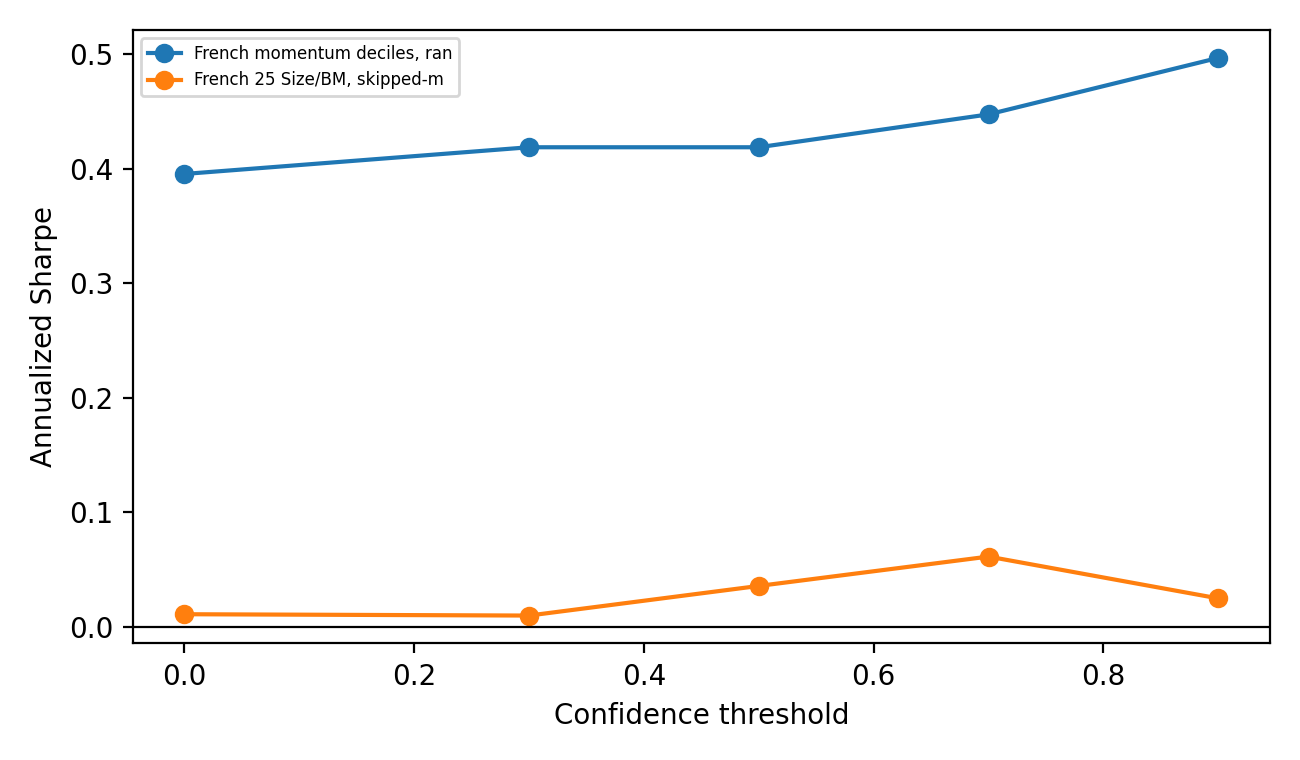
\includegraphics[width=0.82\textwidth]{generated_figures/threshold_profile.png}
\caption{Threshold profile for public candidate panels.}
\label{fig:threshold-profile}
\end{figure}

\begin{figure}[t]
\centering
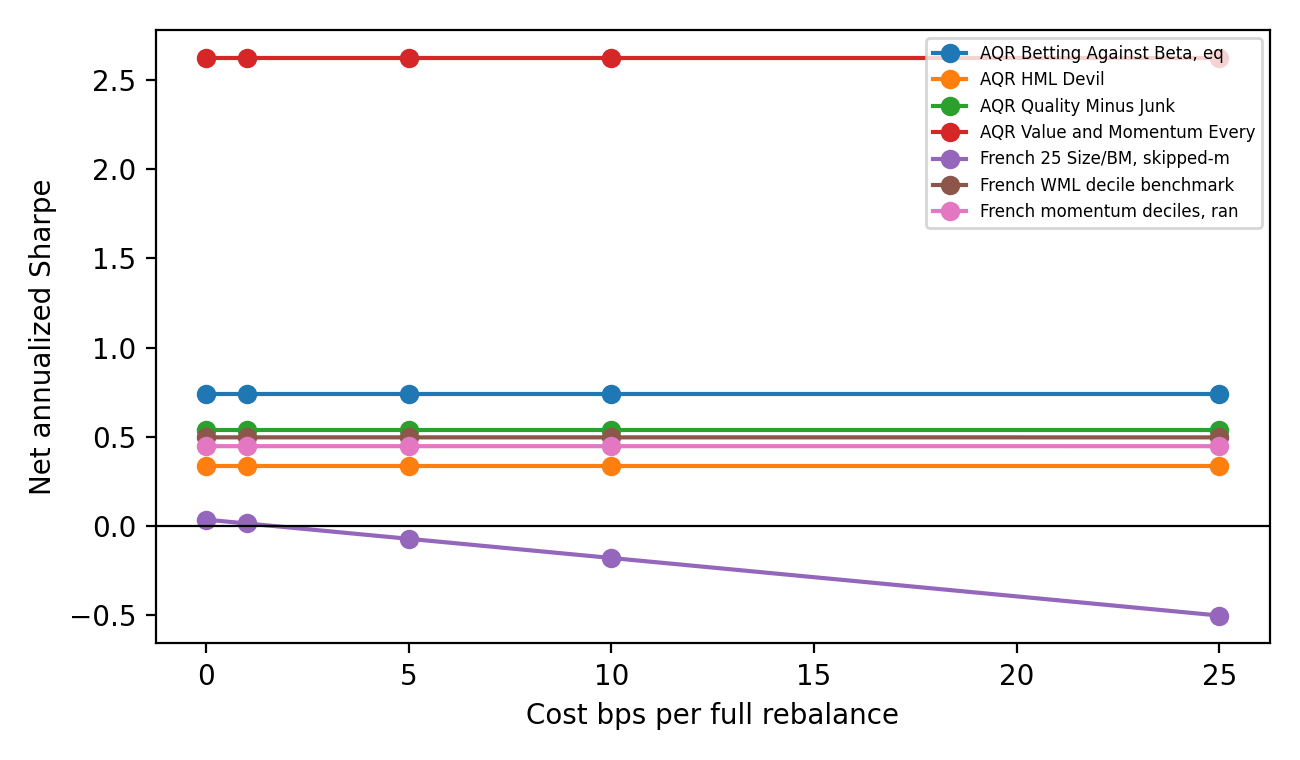
\includegraphics[width=0.82\textwidth]{generated_figures/cost_sensitivity.png}
\caption{Turnover-scaled cost sensitivity at primary candidate thresholds.}
\label{fig:cost-sensitivity}
\end{figure}


\section{Full Monte Carlo Artifacts}

% Generated by render_manuscript_artifacts.py from campaign root code/output_overhaul_20260601


\begin{figure}[t]
\centering
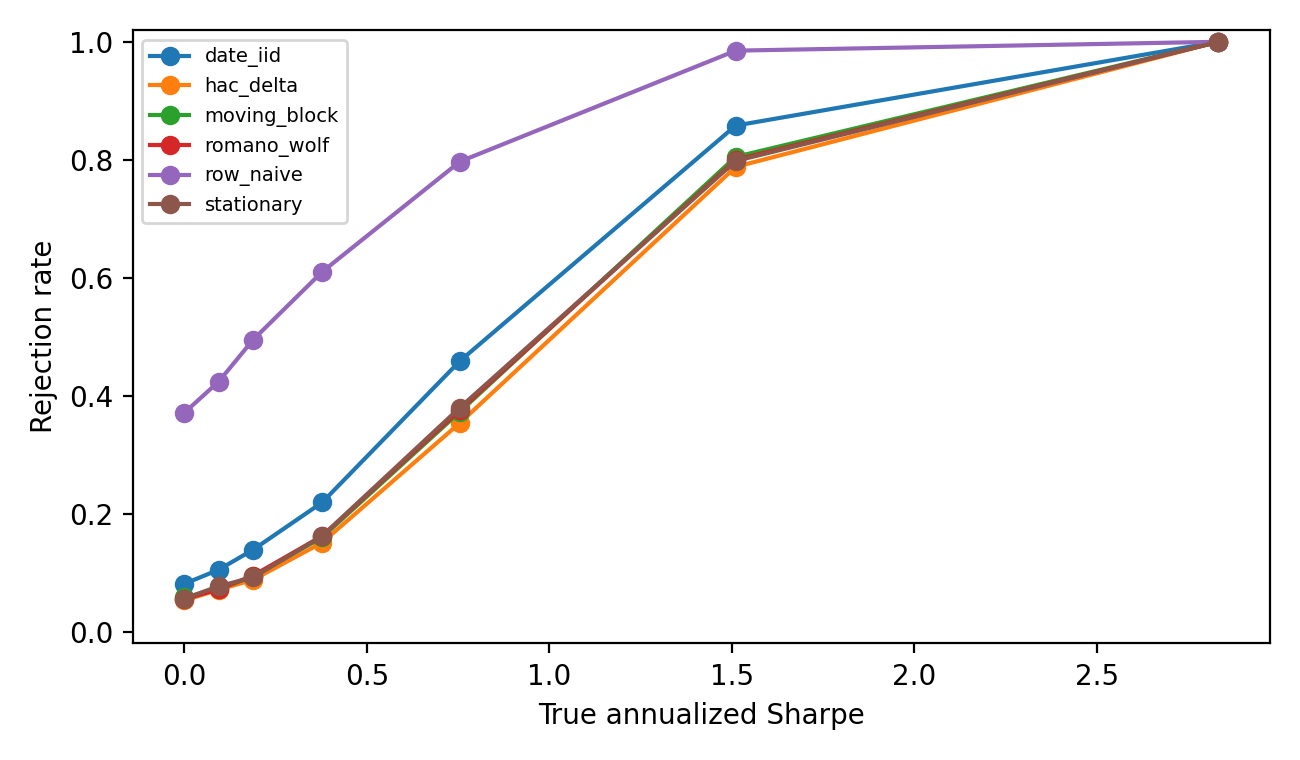
\includegraphics[width=0.82\textwidth]{generated_figures/power_curve.png}
\caption{Monte Carlo rejection rates by true annualized Sharpe.}
\label{fig:power-curve}
\end{figure}

\begin{table}[t]
\centering
\small
\caption{Simulation DGP parameter grid.}
\label{tab:dgp-grid}
\resizebox{\textwidth}{!}{%
\begin{tabular}{llllllllllll}
\toprule
DGP & Name & T & N & mu & sigma & AR1 & rho & GARCH a & GARCH b & K & regime \\
\midrule
01\_iid & IID baseline & 1000 & 50 & 4.00e-04 & 0.015 & 0.000 & 0.000 & 0.000 & 0.000 & 1 & no \\
02\_ser\_mild & Serial mild & 1000 & 50 & 4.00e-04 & 0.015 & 0.200 & 0.000 & 0.000 & 0.000 & 1 & no \\
03\_ser\_strong & Serial strong & 1000 & 50 & 4.00e-04 & 0.015 & 0.500 & 0.000 & 0.000 & 0.000 & 1 & no \\
04\_xs\_mild & Cross mild & 1000 & 50 & 4.00e-04 & 0.015 & 0.000 & 0.200 & 0.000 & 0.000 & 1 & no \\
05\_xs\_strong & Cross strong & 1000 & 50 & 4.00e-04 & 0.015 & 0.000 & 0.500 & 0.000 & 0.000 & 1 & no \\
06\_both\_mod & Both moderate & 1000 & 50 & 4.00e-04 & 0.015 & 0.200 & 0.200 & 0.000 & 0.000 & 1 & no \\
07\_both\_strong & Both strong & 1000 & 50 & 4.00e-04 & 0.015 & 0.500 & 0.500 & 0.000 & 0.000 & 1 & no \\
08\_realistic & Realistic & 2500 & 100 & 4.00e-04 & 0.015 & 0.150 & 0.350 & 0.000 & 0.000 & 1 & no \\
09\_garch\_mild & GARCH mild & 1000 & 50 & 4.00e-04 & 0.015 & 0.200 & 0.200 & 0.050 & 0.900 & 1 & no \\
10\_garch\_strong & GARCH strong & 1000 & 50 & 4.00e-04 & 0.015 & 0.300 & 0.400 & 0.100 & 0.850 & 1 & no \\
11\_multifactor & Multi-factor K=3 & 1000 & 50 & 4.00e-04 & 0.015 & 0.200 & 0.300 & 0.000 & 0.000 & 3 & no \\
12\_regime & Regime-switching & 2000 & 50 & 4.00e-04 & 0.015 & 0.150 & 0.250 & 0.000 & 0.000 & 1 & yes \\
13\_high\_ar1 & High-persistence AR(1) & 1000 & 50 & 4.00e-04 & 0.015 & 0.700 & 0.300 & 0.000 & 0.000 & 1 & no \\
14\_garch\_highvol & High-volatility GARCH & 1000 & 50 & 4.00e-04 & 0.015 & 0.200 & 0.300 & 0.150 & 0.800 & 1 & no \\
\bottomrule
\end{tabular}%
}
\end{table}

\begin{table}[t]
\centering
\small
\caption{Monte Carlo 95 percent interval coverage.}
\label{tab:coverage}
\resizebox{\textwidth}{!}{%
\begin{tabular}{llllll}
\toprule
DGP & blocked & hac\_delta & iid & row\_naive & stationary \\
\midrule
01\_iid & 0.947 & 0.952 & 0.951 & 0.000 & 0.947 \\
02\_ser\_mild & 0.938 & 0.943 & 0.898 & 0.000 & 0.936 \\
03\_ser\_strong & 0.921 & 0.934 & 0.734 & 0.000 & 0.919 \\
04\_xs\_mild & 0.950 & 0.950 & 0.952 & 0.073 & 0.950 \\
05\_xs\_strong & 0.934 & 0.938 & 0.942 & 0.262 & 0.938 \\
06\_both\_mod & 0.937 & 0.939 & 0.898 & 0.088 & 0.936 \\
07\_both\_strong & 0.934 & 0.943 & 0.771 & 0.178 & 0.935 \\
08\_realistic & 0.937 & 0.941 & 0.901 & 0.107 & 0.937 \\
09\_garch\_mild & 0.926 & 0.940 & 0.877 & 0.110 & 0.930 \\
10\_garch\_strong & 0.926 & 0.948 & 0.862 & 0.199 & 0.927 \\
11\_multifactor & 0.937 & 0.947 & 0.895 & 0.225 & 0.940 \\
12\_regime & 0.929 & 0.934 & 0.890 & 0.306 & 0.929 \\
13\_high\_ar1 & 0.899 & 0.933 & 0.562 & 0.137 & 0.907 \\
14\_garch\_highvol & 0.940 & 0.948 & 0.895 & 0.193 & 0.941 \\
\bottomrule
\end{tabular}%
}
\end{table}

\begin{table}[t]
\centering
\small
\caption{Null rejection rates at nominal 5 percent size.}
\label{tab:size}
\resizebox{\textwidth}{!}{%
\begin{tabular}{lllllll}
\toprule
dgp & date\_iid & hac\_delta & moving\_block & romano\_wolf & row\_naive & stationary \\
\midrule
null\_dep & 0.094 & 0.066 & 0.070 & 0.068 & 0.352 & 0.067 \\
null\_garch & 0.098 & 0.063 & 0.070 & 0.067 & 0.351 & 0.068 \\
null\_iid & 0.060 & 0.060 & 0.061 & 0.060 & 0.062 & 0.062 \\
\bottomrule
\end{tabular}%
}
\end{table}

\begin{table}[t]
\centering
\small
\caption{Power by true annualized Sharpe.}
\label{tab:power}
\resizebox{\textwidth}{!}{%
\begin{tabular}{llllllll}
\toprule
index & true\_sharpe & date\_iid & hac\_delta & moving\_block & romano\_wolf & row\_naive & stationary \\
\midrule
0.000 & 0.000 & 0.081 & 0.053 & 0.058 & 0.055 & 0.371 & 0.056 \\
1.000 & 0.094 & 0.105 & 0.071 & 0.072 & 0.072 & 0.424 & 0.077 \\
2.000 & 0.189 & 0.139 & 0.088 & 0.094 & 0.095 & 0.495 & 0.092 \\
3.000 & 0.378 & 0.219 & 0.151 & 0.160 & 0.162 & 0.610 & 0.162 \\
4.000 & 0.755 & 0.459 & 0.354 & 0.373 & 0.376 & 0.797 & 0.380 \\
5.000 & 1.511 & 0.858 & 0.788 & 0.805 & 0.800 & 0.985 & 0.798 \\
6.000 & 2.833 & 1.000 & 1.000 & 1.000 & 1.000 & 1.000 & 1.000 \\
\bottomrule
\end{tabular}%
}
\end{table}


\section{Robustness and Registry Notes}

The public registry is frozen in \path{code/campaign_registry.json}.  It
records loaders, public source metadata, threshold menus, primary
thresholds, and lookback/skip parameters.  Changing a source, lookback,
threshold, cost assumption, or eligibility rule after seeing results
creates a new researcher menu and must be reported as exploratory.

Stationarity diagnostics, holdout splits, HAC bandwidth sweeps,
prewhitened HAC, fixed-fraction HAC, moving-block bootstrap, and
stationary bootstrap results are secondary robustness checks.  They are
used to identify fragile claims, not to replace the main date-return
decision boundary.

\end{document}
